\documentclass[11pt]{article}
\usepackage[margin=1in]{geometry}
\usepackage{amsmath,amssymb}
\usepackage{booktabs,multirow}
\usepackage{graphicx}
\usepackage{natbib}
\usepackage{setspace}
\usepackage[hidelinks]{hyperref}
\usepackage{caption}
\usepackage{longtable}
\newcommand{\champForecastLL}{0.324}
\newcommand{\champForecastAcc}{86.2}
\newcommand{\champContestedAcc}{85.1}
\newcommand{\champAPRE}{0.48}
\newcommand{\incForecastLL}{0.348}
\newcommand{\champGain}{0.024}
\newcommand{\champCongressoutLL}{0.643}
\newcommand{\majorityCongressoutLL}{0.617}
\newcommand{\gbRawForecastLL}{0.803}
\newcommand{\prospectiveVoneLL}{0.331}
\newcommand{\prospectiveVoneAcc}{85.7}
\newcommand{\prospectiveVtwoLL}{0.332}
\newcommand{\prospectiveVtwoAcc}{86.8}
\newcommand{\prospectiveN}{9,451}
\newcommand{\regimeAbestLL}{0.153}

% auto-generated context
\newcommand{\ukRoll}{1235}
\newcommand{\ukDate}{2024-12-20}
\newcommand{\ukCut}{3.44}
\newcommand{\ukDiscrim}{-1.11}
\newcommand{\ukYeaShare}{92}
\newcommand{\ukNPred}{400}

\newcommand{\revoltProbeR}{0.25}
\newcommand{\revoltProbeN}{944}
\newcommand{\ssfaAUCtext}{0.74}
\newcommand{\ssfaDefectors}{71}
\newcommand{\ssfaAUCnotext}{0.69}

\newcommand{\seenLLchamp}{0.504}
\newcommand{\freshLLchamp}{0.300}
\newcommand{\seenLLnotext}{0.590}
\newcommand{\freshLLnotext}{0.421}
\newcommand{\seenLLclean}{0.518}
\newcommand{\freshLLclean}{0.325}
\newcommand{\seenRC}{368}
\newcommand{\freshRC}{1,911}
\newcommand{\houseLLchamp}{0.306}
\newcommand{\senateLLchamp}{0.464}
\newcommand{\houseLLnotext}{0.434}
\newcommand{\senateLLnotext}{0.480}

\newcommand{\ablOrigLL}{0.328}
\newcommand{\ablOrigAUC}{0.78}
\newcommand{\ablShuffLL}{0.392}
\newcommand{\ablShuffAUC}{0.78}
\newcommand{\ablNoSumLL}{0.351}
\newcommand{\ablNoQLL}{0.383}
\newcommand{\ablNoPropLL}{0.339}
\newcommand{\ablGenTitleLL}{0.340}
\newcommand{\ablRC}{1,957}

\newcommand{\brierChamp}{0.099}
\newcommand{\eceChamp}{0.017}
\newcommand{\defShareRChamp}{0.34}
\newcommand{\brierClean}{0.107}
\newcommand{\eceClean}{0.021}
\newcommand{\defShareRClean}{0.32}
\newcommand{\brierNotext}{0.147}
\newcommand{\eceNotext}{0.028}
\newcommand{\defShareRNotext}{0.27}
\newcommand{\defShareNrc}{995}

\newcommand{\overlapRho}{0.05}
\newcommand{\overlapN}{659}
\newcommand{\paulDefGainPct}{77}
\newcommand{\amashDefGainPct}{73}

\newcommand{\cfAraOrig}{6.5}
\newcommand{\cfAraGeneric}{2.7}
\newcommand{\cfAraPassage}{13.5}
\newcommand{\cfAraBio}{8.4}
\newcommand{\cfArdaOrig}{14.5}
\newcommand{\cfArdaCut}{14.7}
\newcommand{\cfArdaGeneric}{12.6}
\newcommand{\cfArdaSwap}{7.3}

\newcommand{\cutHiDiscR}{0.70}
\newcommand{\cutHiDiscMAE}{0.35}
\newcommand{\cutPassageR}{0.61}
\newcommand{\cutPassageMAE}{0.82}

\newcommand{\paulHeldoutN}{949}
\newcommand{\amashHeldoutN}{579}

\newcommand{\covsummaryChamp}{0.327}
\newcommand{\covtitleonlyChamp}{0.286}
\newcommand{\covdesconlyChamp}{0.370}
\newcommand{\covsummaryNotext}{0.444}
\newcommand{\covtitleonlyNotext}{0.439}
\newcommand{\covdesconlyNotext}{0.377}

\newcommand{\omarDefections}{12}
\newcommand{\omarPctChamp}{92}
\newcommand{\omarPctNotext}{93}
\newcommand{\tlaibDefections}{17}
\newcommand{\tlaibPctChamp}{96}
\newcommand{\tlaibPctNotext}{95}
\newcommand{\bushDefections}{9}
\newcommand{\bushPctChamp}{99}
\newcommand{\bushPctNotext}{92}
\newcommand{\aocDefections}{15}
\newcommand{\aocPctChamp}{93}
\newcommand{\aocPctNotext}{94}
\newcommand{\massieDefections}{177}
\newcommand{\massiePctChamp}{99}
\newcommand{\massiePctNotext}{98}
\newcommand{\royCDefections}{87}
\newcommand{\royCPctChamp}{99}
\newcommand{\royCPctNotext}{97}


\newcommand{\code}[1]{\texttt{#1}}

\title{Reading the Bills: Technical Memo\\
\large Motivation, Models, Data, and Validation}
\author{Companion to ``Reading the Bills: Text, Votes, and the
Measurement of Congress''}
\date{July 2026}

\begin{document}
\maketitle

\noindent\emph{Purpose.} This memo is a self-contained technical
account of the companion paper's methods, written to be read from
scratch. It begins with the measurement problem and why reading bill
text can improve on the standard approach (\S\ref{sec:motivation}),
then specifies every model mathematically (\S\ref{sec:models}), and
only afterward turns to the data (\S\ref{sec:data}), the evaluation
design (\S\ref{sec:eval}), the measurement layer
(\S\ref{sec:measurement}), the validation and robustness suite
(\S\ref{sec:validation}), and the code (\S\ref{sec:code}). It
reproduces all of the paper's tables and figures, generated by the
same scripts from the same output files; no statistic in either
document is transcribed by hand. Section references of the form
\code{NN\_name.py} point to the \code{Code/} directory of the
replication repository,
\url{https://github.com/andybhall/reading-the-bills}.

\tableofcontents

%=====================================================================
\section{Motivation}
\label{sec:motivation}

\subsection{The standard model and what it ignores}

Almost every quantitative description of Congress---ideal points,
party unity, NOMINATE dimensions, issue scales---derives from a model
of the form
\begin{equation}
\Pr(y_{iv} = 1) \;=\; \sigma\!\left(\mathbf{a}_v^\top \mathbf{x}_i
+ b_v\right),
\label{eq:classical}
\end{equation}
where $y_{iv}$ is member $i$'s yea/nay vote on rollcall $v$,
$\mathbf{x}_i$ is the member's latent position, and
$(\mathbf{a}_v, b_v)$ are the rollcall's discrimination and difficulty
\citep{poole1997congress, clinton2004statistical}. The object of
interest is usually $\mathbf{x}_i$. The rollcall parameters
$(\mathbf{a}_v, b_v)$ are nuisance parameters: free numbers, one set
per rollcall, estimated from the very votes they are meant to
describe. The bill itself---its text, what the vote is actually
about---never enters the model. Rollcall $v$ is an index.

This design is deliberate and, for estimating $\mathbf{x}_i$, it
works. But treating each bill as a free parameter estimated from its
own votes has two consequences that limit what the measurement
enterprise can do.

\emph{First, the model is silent before the vote.} Because
$(\mathbf{a}_v, b_v)$ are identified only from rollcall $v$'s realized
votes, (\ref{eq:classical}) says nothing about a bill until after it
has been voted on. One cannot ask where a pending bill will divide the
chamber, or which members it will split, because the parameters that
would answer do not yet exist. The bill-location literature
\citep{peress2013estimating, richman2011parties} recovers proposal and
status-quo positions, but still only from realized votes plus
auxiliary structure---after the fact, by construction.

\emph{Second, the free rollcall parameters absorb everything, so
anomalies register as mismeasurement.} A single member position and a
per-rollcall pair of free parameters must reconcile every vote. When a
member defects for a reason one latent dimension cannot hold---a
protest vote against a bill she prefers, a procedural objection, an
ends-against-the-middle alignment with the opposite pole---the model
has no structural place to put it, and either mis-locates the member
or treats the vote as noise. A decade of scaling research has built
bespoke models for exactly these cases: heteroskedastic ``unpredictable
voter'' terms \citep{lauderdale2010unpredictable}, non-monotone
response functions \citep{duckmayr2023ends}, and protest-vote mixtures
\citep{fowler2026protest}.

\subsection{The idea: amortize the bill from its text}

Both limitations trace to the same choice: rollcall parameters are
free, estimated per rollcall. Suppose instead we make them a
\emph{function of the bill's pre-vote text},
\begin{equation}
\mathbf{a}_v = g_a(\phi_v), \qquad b_v = g_b(\phi_v),
\label{eq:amortize}
\end{equation}
where $\phi_v$ is a feature vector built from the bill's text (via a
modern language-model embedding) and a little pre-vote metadata, and
$g_a, g_b$ are maps learned across all rollcalls. This is
\emph{amortization}: instead of a private parameter set per rollcall,
one shared map turns any bill's text into its rollcall parameters.
Three things follow immediately.

\begin{enumerate}
\item \textbf{Unseen bills get parameters.} Because $g_a, g_b$ take
text as input, a bill the model has never seen---including one not yet
voted on---receives a discrimination and difficulty, hence a predicted
cutpoint and a member-by-member forecast. Prediction becomes
prospective.
\item \textbf{The text--coalition map is a learnable, testable
object.} $g_a$ encodes how bill content translates into coalition
geometry. If content organizes coalitions in recurring ways---must-pass
fiscal deals splitting a majority's flank, suspension items commanding
consensus---then $g_a$ can learn it, and we can measure how much it
learns out of sample.
\item \textbf{The classical model is the unconstrained limit.}
Equation~(\ref{eq:classical}) is what (\ref{eq:amortize}) becomes when
$g$ is allowed a free output per rollcall. Amortization is therefore a
bet: that constraining rollcall parameters to be a function of text
\emph{improves} out-of-sample prediction over leaving them free, because
text carries real signal and the constraint regularizes. That bet is
falsifiable, and the evaluation regimes of \S\ref{sec:eval} are built
to test it honestly---under temporal holdout, under transfer to unseen
congresses, and under a frozen prospective protocol.
\end{enumerate}

\subsection{Why it can be an improvement, concretely}

The bet pays off along three measurable dimensions, which structure
the companion paper and the measurement layer of \S\ref{sec:measurement}.

\begin{itemize}
\item \emph{Fit.} Even setting text aside, a member model flexible
enough to hold the anomalous cases (higher-dimensional positions plus a
member intercept) beats the classical model on its own held-out
classification statistic, and the gains concentrate on the members
scaling research built bespoke models to rescue
(\S\ref{sec:idealpoint}, Fig.~\ref{fig:membergmp}).
\item \emph{Prospective coalition behavior.} Reading the bill lets the
model anticipate majority-party defections before the vote---the
protest phenomenon that scaling models could previously only
reinterpret after the fact (\S\ref{sec:measurement},
Fig.~\ref{fig:protest}--\ref{fig:capture}).
\item \emph{Prospective location.} Text plus pre-vote metadata
predicts where a bill will cut the chamber before anyone votes
(\S\ref{sec:cutpoints}, Fig.~\ref{fig:cutpred}).
\end{itemize}

\subsection{The discipline the idea requires}

Modern language-model encoders make this program easy to overclaim.
Two hazards recur: \emph{leakage}, where a feature encodes information
not actually available before the vote (a summary revised after the
fact, a subject tag re-coded later), and \emph{reusable-holdout
overfitting}, where iterating on a fixed test set inflates apparent
performance \citep{dwork2015holdout}. A large share of this memo is the
scaffolding that guards against both: a per-field timing audit and a
leakage-clean specification (\S\ref{sec:leakage}), a hash-pinned
prospective protocol scoring frozen models only on later votes
(\S\ref{sec:prospective}), redaction ablations that hold every non-text
input fixed (\S\ref{sec:ablation}), and a pre-registered experiment
ledger (\S\ref{sec:eval}). The models are the easy part; the evaluation
is where the claims are earned.

%=====================================================================
\section{The models}
\label{sec:models}

We predict individual voting decisions: given everything observable
before rollcall $v$, the probability that member $i$ votes yea,
conditional on a recorded yea or nay. This section specifies each model
mathematically. Feature construction (the text template, the encoders,
the joins that build $\phi_v$) is deferred to \S\ref{sec:data}; here
$\phi_v$ is simply ``the pre-vote feature vector for rollcall $v$,''
and the evaluation regimes referenced below are defined in
\S\ref{sec:eval}.

\subsection{Count baselines (\code{models\_forecast.py})}

The simplest models condition on nothing but voting history. Question
buckets partition the \code{vote\_question} string by regular
expression into \{passage, amendment, procedural, cloture, resolution,
nomination, other\}. \code{MemberQuestionRate} predicts member $i$'s
empirical training-window yea rate within the bucket, shrunk toward the
member's overall rate for thin cells, with member~$\to$~global
fallback; \code{PartyQuestionRate} and \code{MajorityQuestionRate} are
the party- and majority-status-keyed analogs. These are the ``count
table'' baselines that the 2011--2016 text models fail to beat
(Table~\ref{tab:lit}), and the member-history table re-appears inside
the two-tower model as an offset (\S\ref{sec:texttower}).

\subsection{Spatial models (\code{models\_idealpoint.py})}
\label{sec:idealpoint}

The $k$-dimensional logistic ideal-point model adds a member intercept
to (\ref{eq:classical}):
\begin{equation}
\Pr(y_{iv} = 1) \;=\; \sigma\!\left(\mathbf{a}_v^\top \mathbf{x}_i
+ b_v + c_i\right),
\label{eq:irt}
\end{equation}
with member position $\mathbf{x}_i \in \mathbb{R}^k$, member intercept
$c_i$ (base yea propensity), and rollcall parameters
$(\mathbf{a}_v, b_v)$ indexed by (congress, chamber, rollnumber). It is
estimated by minibatch AdamW (learning rate $.05$, weight decay
$10^{-4}$, batch $2^{17}$, at most 60 epochs) on binary cross-entropy.
Weight decay is a ridge penalty, i.e.\ independent Gaussian MAP
shrinkage on all parameters. Early stopping (patience 3) uses an
internal 2\% hash-keyed slice of \emph{train}---never the benchmark
validation or test sets. Initialization:
$\mathbf{x}, \mathbf{a} \sim N(0, .1^2)$, $b = c = 0$; where used,
dimension~1 of $\mathbf{x}$ is seeded at $\pm 0.5$ by party
(party-sign initialization), which selects the optimization basin---so
the learned first axis cannot flip orientation across eras---without
constraining what the data can express. Unseen members predict at
$\mathbf{x} = 0, c = 0$; unseen rollcalls (impossible in the completion
regime) fall back to the global training rate.

\code{NominateLogit} is the classical reference: positions frozen at
two-dimensional DW-NOMINATE scores, with only $(\mathbf{a}_v, b_v)$
estimated, by the same optimizer on the same cells. Because both models
estimate rollcall parameters on training cells only and are scored on
cells neither saw, the member-level comparison
(Fig.~\ref{fig:membergmp}, Table~\ref{tab:hardcase},
\code{24\_member\_fit.py}) isolates what flexible positions add over
frozen ones under an identical likelihood and estimator.

\paragraph{Identification.} The likelihood of (\ref{eq:irt}) is
invariant to affine maps of the latent space. For prediction this is
irrelevant; for the measurement layer, positions are standardized
within chamber-congress (mean 0, variance 1) and oriented so the
Republican mean exceeds the Democratic mean, and all cutpoints,
screens, and directions are stated on that scale
(\S\ref{sec:cutpoints}).

\paragraph{Relation to existing estimators.} Equation~(\ref{eq:irt})
with $k = 1$ and $c_i = 0$ is exactly the two-parameter logistic IRT
model of \citet{clinton2004statistical}; the member intercept $c_i$ and
$k > 1$ are strict generalizations, so the model \emph{nests} the
canonical Bayesian spatial model (point-estimated here rather than
sampled, with weight decay standing in for the prior). Relative to
NOMINATE \citep{poole1997congress}, the response function differs
(logistic in a linear utility difference rather than normal/GEV in
Gaussian deterministic utilities), which is why the frozen-position
bridge model \code{NominateLogit} is used for all head-to-head
comparisons rather than published NOMINATE classifications. Relative to
\citet{imai2016fast}, estimation is SGD on the full likelihood rather
than EM on a variational bound---the same scalability goal by different
means. The member intercept plus $k = 8$ dimensions absorb, in reduced
form, phenomena that dedicated models capture structurally:
member-specific error rates \citep{lauderdale2010unpredictable},
ends-against-the-middle response functions \citep{duckmayr2023ends}
(GGUM's non-monotone single-dimension response is representable as a
monotone response in a higher-dimensional space), and protest-vote
mixtures \citep{fowler2026protest}. The completion-regime results
quantify how much of those phenomena reduced-form flexibility recovers
(most of it, for fit purposes); the defection-forecasting layer then
addresses what those models' substantive target---the anomalous
votes---looks like prospectively.

\subsection{The two-tower text model (\code{models\_texttower.py})}
\label{sec:texttower}

The forecasting architecture is the amortization idea of
(\ref{eq:amortize}) made concrete. It replaces the free rollcall
parameters of (\ref{eq:irt}) with parameters computed from pre-vote
features, so that never-before-seen rollcalls receive predictions:
\begin{equation}
\operatorname{logit}\Pr(y_{iv}=1) \;=\;
\underbrace{g_a(\phi_v)^\top \mathbf{x}_i}_{\text{amortized
discrimination}} \;+\; \underbrace{g_b(\phi_v)}_{\text{amortized
difficulty}} \;+\; c_i \;+\;
\boldsymbol\gamma^\top \mathbf{z}_{iv},
\label{eq:tower}
\end{equation}
with $\mathbf{x}_i \in \mathbb{R}^{16}$ and $c_i$ member parameters as
in (\ref{eq:irt}). The name is literal: one ``tower'' maps the bill's
features $\phi_v$ to rollcall parameters, the other holds the member
vector $\mathbf{x}_i$, and they meet in the bilinear term.

\paragraph{Rollcall features $\phi_v$.} The concatenation of
(i)~the sentence embedding of the rollcall text template
(\S\ref{sec:template}), rescaled by $5$ (embeddings are unit-norm; the
rescale matches their variance to the other blocks)---or, in the
TF--IDF component, a 30{,}000-feature (1--2)-gram sublinear TF--IDF of
title + policy area + subjects, SVD-compressed to 128 dimensions and
per-dimension standardized; (ii)~question-bucket one-hots;
(iii)~bill-category one-hots; (iv)~sponsor-party indicators. The
no-text counterpart deletes block~(i) only, and is otherwise the same
model---the counterfactual for ``what does reading the bill add.''

\paragraph{Heads.} $g_a: \mathbb{R}^d \to \mathbb{R}^{16}$ and
$g_b: \mathbb{R}^d \to \mathbb{R}$ are two-layer MLPs (width 128, ReLU)
in the \code{mlp\_head} variants, linear maps otherwise. The MLP lets
text dimensions interact before meeting the member vector.

\paragraph{Member--rollcall covariates $\mathbf{z}_{iv}$.} Same-party
and opposite-party indicators between the member and the bill sponsor,
plus the logit of the member $\times$ question-bucket empirical
training rate---the count baseline of the previous subsection entering
as an offset with learned weight, initialized at 1 (``trust the
empirical rate, then improve on it'').

\paragraph{Training.} AdamW (lr $.02$, weight decay $10^{-4}$), batch
$2^{17}$, at most 60 epochs, patience 5 with a 10-epoch minimum
(bilinear terms move slowly at first; stopping earlier was
device-RNG-dependent, a diagnosed failure mode). The internal
development slice for early stopping is \emph{temporal}: the final 5\%
of training rollcalls by date within each congress-chamber, whole
rollcalls, strictly inside train. A random-cell slice---in-sample for
rollcall parameters---was shown to miscalibrate forecast models (82\%
accuracy at 0.64 log loss in the diagnostic that motivated the change);
the temporal slice sees future-like data.

\paragraph{Calibration.} Post-hoc temperature and bias
$(\tau, \beta_0)$, fit by L-BFGS on the development slice:
$\operatorname{logit} p \mapsto \operatorname{logit} p / \tau +
\beta_0$. Per-question-bucket calibration was tested and rejected
(ledger~E3).

\paragraph{Ensembling.} \code{LogitBlend} is a logistic regression on
component logits---weights and bias only, fit by L-BFGS on the same
development slice, initialized at unit weight on the first component.
Weights are unconstrained (they need not sum to one); redundant
components collapse toward zero, the pre-registered falsification
criterion of ledger~E4. The champion \code{blend3\_mlp\_tfidf\_emb3\_tcal}
combines (1) the MiniLM-MLP tower, (2) the MiniLM + TF--IDF linear
tower, and (3) the Qwen-MLP tower, with fitted weights
$0.57/0.12/0.42$. The no-text counterfactual \code{notext\_mq\_16d\_tcal}
is the champion architecture with block~(i) deleted,
\emph{independently} trained, early-stopped, and calibrated---nothing
is inherited from text models.

\paragraph{Relation to existing models.} Equation~(\ref{eq:tower}) is
the modern-encoder descendant of the 2011--2016 program.
\citet{gerrish2011predicting} regress rollcall parameters on LDA topics
jointly with an ideal-point model; the two-tower model differs in
(a)~representation (frozen sentence-transformer embeddings or
TF--IDF/LSA instead of LDA), (b)~estimation (joint SGD of member and
amortization parameters, rather than a topic model in the loop), and
(c)~the member-history offset, which the earlier literature lacked and
which our results show is the binding baseline. Our reimplementation
(\S\ref{sec:litreimpl}) preserves their two-stage logic exactly so that
the representation upgrade can be isolated (\code{gb\_spatial\_emb2}
swaps embeddings into their architecture). \citet{kraft2016embedding}
is the closest architectural relative: a bilinear form between a learned
member embedding and a linear map of a fixed text embedding, plus member
intercept. The two-tower model \emph{nests} it: setting the head linear,
removing metadata blocks from $\phi_v$, and removing $\mathbf{z}_{iv}$
and the calibration recovers the Kraft bilinear core (this is precisely
our \code{kraft\_bilinear\_16d} reimplementation). The additions that
matter empirically, in ledger order, are the member-history offset, the
temporal development slice with calibration, and the MLP head.
Amortization of item parameters from covariates also connects to the
structured-IRT tradition; the distinctive commitments here are
pre-vote-only text, a benchmark harness with temporal separation, and
frozen encoders (no fine-tuning, ledger~M-A).

\subsection{Reimplemented literature baselines
(\code{models\_litbaselines.py})}
\label{sec:litreimpl}

\textbf{GBSpatial} (Gerrish--Blei analog, two stage): stage~1 fits the
1-D version of (\ref{eq:irt}) on training votes; stage~2 ridge-regresses
each rollcall's $(a_v, b_v)$ on its text representation
(TF--IDF$\to$SVD, or sentence embeddings in the \code{emb2} variant),
with the ridge penalty chosen on an internal 10\% slice of training
rollcalls by downstream vote log loss. Evaluation rollcalls receive
text-predicted parameters against train-fitted member positions.
Reported as published and with temperature calibration added
(\code{gb\_*\_tcal}), which the original lacks. \textbf{Kraft bilinear}:
as above; documented deviations, all favoring the baseline: modern
sentence embeddings for averaged word2vec, a sponsor-alignment term,
$k = 16$ matching the champion, and the temporal early-stopping
discipline. \textbf{NOMINATE-context logit}: frozen DW-NOMINATE
interacted with congress, question bucket, and sponsor
alignment---the strongest ``classical scores plus metadata, no text''
null. Voteview scores are career-based and thus see evaluation-period
votes; this accepted advantage to the baseline is flagged wherever the
model appears.

\begin{table}[tbp]
\centering
\caption{Temporal-forecast comparison (identical evaluation; right
panel: congress-out transfer). Generated by \code{make\_tables.py} from
the benchmark leaderboard.}
\label{tab:regime}
\begin{tabular}{lcccc}
\toprule
Information used & \multicolumn{2}{c}{Temporal forecast} & \multicolumn{2}{c}{Congress-out} \\
\midrule
Party history only & 0.466 & 76.6 & 0.693 & 57.1 \\
Member history only & 0.459 & 76.0 & 0.693 & 57.1 \\
Rollcall metadata only & 0.511 & 72.3 & 0.717 & 58.6 \\
Text + metadata (no member history) & 0.464 & 77.8 & 0.741 & 64.4 \\
Text + metadata + member history & 0.411 & 80.1 & 0.720 & 59.3 \\
+ modern encoder, deep head, calibration & 0.348 & 85.2 & 0.670 & 61.6 \\
+ ensemble (final) & 0.324 & 86.2 & 0.643 & 62.1 \\
\bottomrule
\end{tabular}

\end{table}

\begin{table}[tbp]
\centering
\caption{The 2011--2016 architectures and count baselines under
identical information rules.}
\label{tab:lit}
{\footnotesize \begin{tabular}{lccccc}
\toprule
Model & Fcst.\ LL & Fcst.\ AUC & Fcst.\ cont.\ acc.\ (\%) & Rand.\ LL & Rand.\ AUC \\
\midrule
Constant rate & 0.617 & 0.500 & 52.7 & 0.659 & 0.500 \\
Party $\times$ question rate & 0.466 & 0.805 & 69.8 & 0.504 & 0.797 \\
Member $\times$ question rate & 0.459 & 0.812 & 69.2 & 0.494 & 0.807 \\
NOMINATE $\times$ context logit & 0.532 & 0.740 & 59.6 & 0.587 & 0.713 \\
GB-style spatial (TF-IDF) & 0.803 & 0.689 & 57.6 & 1.054 & 0.687 \\
GB-style spatial (TF-IDF, calibrated) & 0.566 & 0.689 & 57.1 & 0.685 & 0.687 \\
GB-style spatial (mod.\ emb., calibrated) & 0.556 & 0.699 & 55.8 & 0.662 & 0.670 \\
Kraft-style bilinear & 0.497 & 0.790 & 67.2 & 0.522 & 0.794 \\
TF-IDF tower + member offset & 0.411 & 0.860 & 75.0 & 0.448 & 0.854 \\
MiniLM-MLP tower (prior champion) & 0.348 & 0.906 & 84.0 & 0.417 & 0.880 \\
Three-tower blend (champion) & 0.324 & 0.919 & 85.1 & 0.390 & 0.896 \\
\bottomrule
\end{tabular}
}
\end{table}

\begin{table}[tbp]
\centering
\caption{Completion-regime ladder (psychometric setting).}
\label{tab:regimeA}
\begin{tabular}{lcccc}
\toprule
Model & Log loss & Acc.\ (\%) & Contested acc.\ (\%) & APRE \\
\midrule
Constant rate & 0.655 & 63.7 & 50.9 & -0.32 \\
Member rate & 0.629 & 64.9 & 55.2 & -0.28 \\
Party $\times$ rollcall majority & 0.206 & 91.7 & 92.8 & 0.70 \\
Ideal points (1D) & 0.193 & 91.6 & 91.2 & 0.69 \\
DW-NOMINATE logit (frozen scores) & 0.164 & 93.3 & 93.9 & 0.76 \\
Ideal points (2D) & 0.161 & 93.3 & 93.8 & 0.76 \\
Ideal points (8D) & 0.153 & 93.8 & 94.3 & 0.77 \\
\bottomrule
\end{tabular}

\end{table}

%=====================================================================
\section{Data}
\label{sec:data}

\subsection{Sources}

\begin{itemize}
\item \textbf{Voteview} \citep{lewis2026voteview}: members, rollcalls,
and individual votes for the 101st--119th Congresses
(\code{00\_download\_data.py}); DW-NOMINATE and Nokken--Poole scores for
the frozen-position baselines and convergent-validity checks. Data
snapshot: June 9, 2026 (pinned in the frozen-model metadata; see
\S\ref{sec:prospective}).
\item \textbf{GovInfo BILLSTATUS} bulk XML
(\code{05\_fetch\_billstatus.py}, \code{07\_parse\_bills.py}): bill
titles, sponsors, policy areas, legislative subjects, and dated summary
versions, available from the 108th Congress onward. Amendment records
(\code{18\_parse\_amendments.py}): amendment sponsor, party, purpose
text, submission date. Cosponsorship records with sponsorship dates
(\code{16\_parse\_cosponsors.py}).
\end{itemize}

Raw downloads are never modified; every transformation is code that
writes to \code{Modified Data/}.

\subsection{Panel construction}

\code{01\_build\_votes.py} converts Voteview cast codes to binary
yea/nay (paired/announced positions follow Voteview's coding; abstains
and absences are excluded), yielding 10.6M member--vote decisions. The
unit of analysis is the member--rollcall cell $(i, v)$ with outcome
$y_{iv} \in \{0, 1\}$. Table~\ref{tab:benchcard} is the benchmark card:
composition by congress block and chamber, bill-linkage and
text-coverage shares, and holdout performance by coverage cell.

\begin{table}[tbp]
\centering
\caption{Benchmark card (script \code{37\_benchmark\_card.py}).
``Bill-linked'' is the share of rollcalls tied to a legislative
measure; ``pre-vote summary'' the share whose leakage-clean text
template draws on a CRS summary dated strictly before the vote; ``title
only'' the share whose bill text is a title.}
\label{tab:benchcard}
{\footnotesize \begin{tabular}{llccccc}
\toprule
Congresses & Chamber & Rollcalls & \shortstack{Member\\votes} & \shortstack{Bill-\\linked} & \shortstack{Pre-vote\\summary} & \shortstack{Title\\only} \\
\midrule
101--107 (pre-text era) & House & 7,560 & 3,122,125 & 0\% & 0\% & 0\% \\
101--107 (pre-text era) & Senate & 4,748 & 462,932 & 0\% & 0\% & 0\% \\
108--113 & House & 8,744 & 3,615,380 & 97\% & 94\% & 3\% \\
108--113 & Senate & 3,816 & 367,139 & 80\% & 79\% & 1\% \\
114--119 & House & 6,288 & 2,622,471 & 97\% & 71\% & 26\% \\
114--119 & Senate & 4,286 & 411,954 & 45\% & 37\% & 8\% \\
\midrule
\multicolumn{7}{l}{\emph{Temporal-holdout log loss by text coverage:}} \\
\multicolumn{3}{l}{} & Member votes & \multicolumn{2}{c}{Champion} & No-text \\
\multicolumn{3}{l}{\quad Summary-bearing rollcalls} & 552,219 & \multicolumn{2}{c}{0.327} & 0.444 \\
\multicolumn{3}{l}{\quad Title-only rollcalls} & 92,854 & \multicolumn{2}{c}{0.286} & 0.439 \\
\multicolumn{3}{l}{\quad Description-only or unlinked} & 44,278 & \multicolumn{2}{c}{0.370} & 0.377 \\
\bottomrule
\end{tabular}
}
\end{table}

\subsection{Bill linkage and the amendment-records join}

\code{04\_link\_bills.py} links rollcalls to measures via Voteview's
bill-number field, normalized to (congress, bill type, bill number);
\code{bill\_category} distinguishes legislation from nominations,
resolutions of ratification, and unlinked votes. Amendment rollcalls
pose a mapping problem: clerk roll numbers reset each session while
Voteview numbers cumulate within a congress. The join in
\code{18\_parse\_amendments.py} therefore adds explicit first-session
roll-count offsets per (congress, chamber) and verifies every matched
pair by date equality; an earlier draft that ignored the offset
produced zero test-window matches with 367-day date gaps, which is the
failure mode the verification now guards against. Coverage:
\amdtTotal{} amendment rollcalls, of which \amdtNoDesc{} lack any
descriptive text from Voteview and \amdtFilledNoDesc{} of those gain
amendment-side information (sponsor, party, purpose) through the join;
amender-party coverage on matched amendment rollcalls is
\amdtSponsorCov\%.

\subsection{The rollcall text template and $\phi_v$}
\label{sec:template}

\code{08\_embed\_bills.py} composes, for every rollcall, the exact text
the sentence encoders see:
\begin{center}
\code{vote\_question. vote\_desc. bill\_text}
\end{center}
truncated to 1{,}500 characters (MiniLM tower) or 6{,}000 characters
(Qwen tower), where \code{bill\_text} is the latest CRS summary whose
action date is \emph{strictly earlier} than the vote date, else the
bill title, else empty. The \code{text\_source} flag
(\code{summary}/\code{title}/\code{desc\_only}/\code{none}) drives the
coverage cells of Table~\ref{tab:benchcard}. Two encoders are used:
\code{all-MiniLM-L6-v2} (384-d, frozen) produces the v2 embedding file,
and \code{Qwen3-Embedding-0.6B} (1{,}024-d) the v3 file;
\code{19\_build\_text\_v4.py} covers the longer-budget variants tested
and rejected in ledger experiment~M-A. All embeddings are
$\ell_2$-normalized. The embedding, together with the metadata one-hots
of \S\ref{sec:texttower}, is the feature vector $\phi_v$ that enters
(\ref{eq:tower}).

Two fields are generated at the vote itself and admit no earlier
timestamp: the Clerk's vote-question and vote-description strings. The
redaction ablations of \S\ref{sec:ablation} bound their contribution. A
separate TF--IDF block used by one ensemble component draws on bill
title + policy area + legislative subjects; subjects are CRS-curated and
revisable without version history, which is why the single MiniLM tower
is reported throughout as the fully leakage-clean specification
(\S\ref{sec:leakage}).

%=====================================================================
\section{Evaluation design}
\label{sec:eval}

\subsection{Regimes}
\label{sec:regimes}

All splits are deterministic functions of content-hashed keys or dates;
the evaluation harness (\code{harness.py}, \code{run\_benchmark.py})
strips labels from evaluation rows before models see them.

\begin{enumerate}
\item \textbf{Completion} (\code{regimeA\_seed42},
\code{02\_make\_splits.py}): member--vote cells are assigned to
train/validation/test by a salted SHA-256 hash of (congress, chamber,
rollnumber, icpsr), so held-out votes are missing at random while
same-rollcall votes remain observable---the psychometric setting in
which ideal-point models are traditionally assessed. Covers the
101st--119th Congresses.
\item \textbf{Random-rollcall holdout} (\code{randomrc108\_119},
\code{17\_make\_randomrc\_split.py}): whole rollcalls held out at
random---rollcall parameters cannot be estimated from partial votes, so
this regime requires amortization from features.
\item \textbf{Temporal forecast} (\code{forecast108\_119},
\code{06\_make\_forecast\_split.py}): within each congress-chamber,
rollcalls are ordered by date (roll number breaking ties) and the final
10\% form the test set; the preceding 90\% train. The primary
forecasting regime.
\item \textbf{Congress-out} (\code{congressout118},
\code{12\_make\_congressout\_split.py}): train through the 116th,
validate on the 117th, test on the 118th---the transfer setting whose
results (Table~\ref{tab:regime}, right panel) bound all claims.
\item \textbf{Prospective} (\S\ref{sec:prospective}): hash-pinned
frozen artifacts scored only on votes cast after freezing, following
the reusable-holdout logic of \citet{dwork2015holdout}.
\end{enumerate}

\subsection{Metrics}

With $p_{iv}$ the predicted yea probability (clipped to
$[\varepsilon, 1-\varepsilon]$, $\varepsilon = 10^{-7}$): log loss
$= -\frac{1}{N}\sum y_{iv}\log p_{iv} + (1-y_{iv})\log(1-p_{iv})$;
GMP $= \exp(-\text{log loss})$ \citep{carroll2013structure}; correct
classification $= \frac{1}{N}\sum \mathbf{1}\{(p_{iv} \ge .5) =
y_{iv}\}$; Brier $= \frac{1}{N}\sum (p_{iv}-y_{iv})^2$. APRE is
aggregate proportional reduction in error against each rollcall's own
minority margin: $\text{APRE} = \sum_v (m_v - e_v) / \sum_v m_v$ with
$m_v$ the minority vote count and $e_v$ the classification errors on
rollcall~$v$. AUC uses midranks for ties. The within-vote defection AUC
of \S\ref{sec:measurement} is computed per (rollcall, majority party)
over that party's members with defection ($y=0$) as the positive class,
then averaged with equal weight over rollcalls with at least three
defections (the all-positive-defection version is reported alongside).
Expected calibration error uses 15 equal-count bins
(\code{32\_calibration\_metrics.py}).

\subsection{Uncertainty}

Headline comparisons carry paired rollcall-cluster bootstrap intervals:
rollcalls are resampled with replacement, both models' per-vote losses
are re-averaged on the same resample, and the difference distribution is
summarized by its 2.5/97.5 percentiles (ensemble vs.\ strongest
component: $[\pairedDeltaOneLo, \pairedDeltaOneHi]$ log loss; text vs.\
no-text on the protest task: $[\pairedDeltaTwoLo, \pairedDeltaTwoHi]$).
The prospective v1 interval (\prospLLlo--\prospLLhi) is a
rollcall-cluster bootstrap over the post-snapshot rollcalls.

\subsection{Protocol discipline}

Development followed a pre-registered experiment ledger
(\code{Notes/experiment\_ledger.md}; reproduced as
Table~\ref{tab:ledger}): hypothesis, knowability argument, and
falsification criterion recorded before each experiment's first run;
model selection on validation only; the final three-model comparison
observed test sets once. One operational rule is worth recording: a
same-model, same-input log-loss drift (0.3883 vs.\ 0.4275 on
\code{randomrc}) was traced to deep in-process state after multiple
model fits in one Python process---inputs were hash-verified identical,
fresh-process repeats were bit-identical---so all registered results
come from one-model-per-process runs.

%=====================================================================
\section{The measurement layer}
\label{sec:measurement}

The models above forecast votes; this section turns the forecasts into
the measures of the companion paper.

\subsection{Realized rollcall cutpoints}
\label{sec:cutpoints}

\code{22\_extract\_measures.py} and \code{23\_text\_cutpoints.py} fit
the 1-D version of (\ref{eq:irt}) per chamber-congress (108th--119th),
party-sign initialized, on all votes. A rollcall's \emph{realized
cutpoint} is the position at which the average member is indifferent,
\begin{equation}
x^*_v = -\,(b_v + \bar c)\,/\,a_v,
\end{equation}
standardized by the chamber-congress member distribution, with
direction $\operatorname{sign}(a_v)$ (positive = yeas attract
conservatives), reported when $|a_v| \ge 0.35$ (threshold sensitivity:
the share of cutpoints between the party medians moves only from
\cutBetweenPartiesLo\% to \cutBetweenPartiesHi\% across screens). This
quantity is a property of the realized vote---content, agenda control,
and party pressure together---\emph{not} the proposal or status-quo
location of \citet{peress2013estimating} or \citet{richman2011parties},
which are identified from realized votes plus auxiliary structure. The
distinction runs in both directions: those estimators locate bills after
the vote; the prediction exercise below locates rollcalls before it. No
overlapping-sample comparison with Peress/Richman-style estimates has
been run yet; it is the natural next test and would require
reimplementing those estimators.

\subsection{Predicting cutpoints from pre-vote features}

Within each congress-chamber the first 80\% of rollcalls (by date) train
the predictors and the final 20\% are held out. Location: ridge
regression (penalty by cross-validation inside the training window);
direction: logistic regression. Feature sets: constant; metadata
(question bucket, bill category, chamber, the bill sponsor's party and,
on amendment votes, the amender's party, with interactions);
TF--IDF$\to$SVD of the rollcall text; MiniLM embeddings of the same
text; embeddings + metadata (the headline set; it contains no
CRS-revisable fields). Term-level interpretability uses a sparse model
on final-passage summaries with alphabetic tokens and stop-word and
year-token screens (Fig.~\ref{fig:dirterms})---screens added after
face-validity failures (year tokens proxying majority control;
rules-resolution boilerplate) documented in the session logs.

\begin{figure}[tbp]
\centering
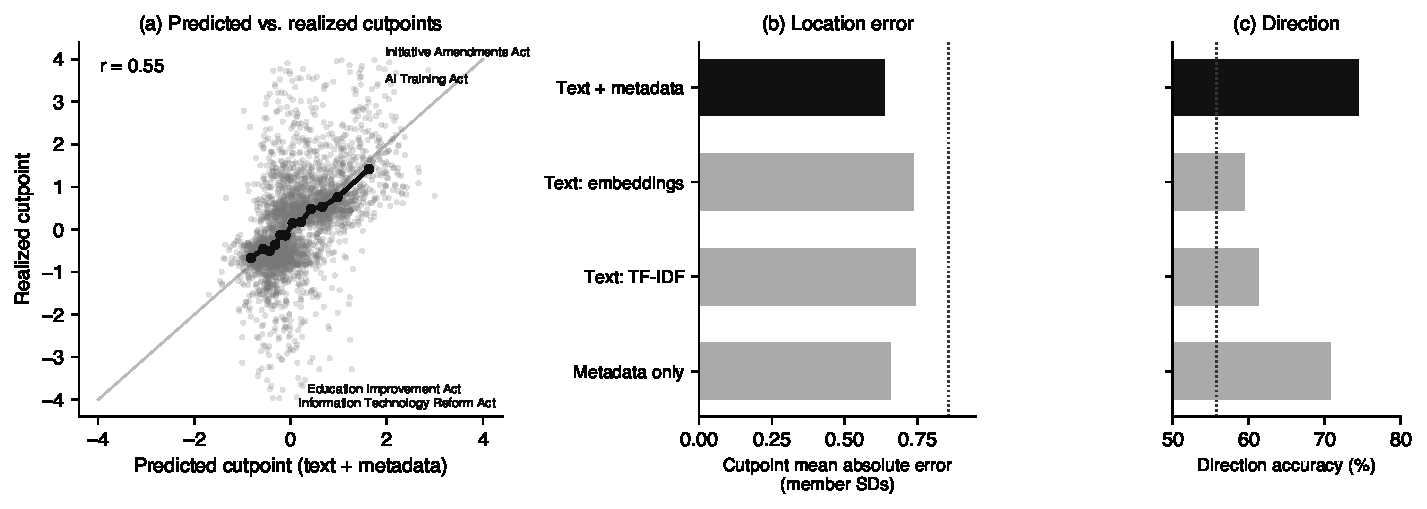
\includegraphics[width=.98\linewidth]{figures/cutpoint_prediction.pdf}
\caption{Cutpoint prediction on held-out rollcalls
(\code{23\_text\_cutpoints.py}, figure \code{f8}).}
\label{fig:cutpred}
\end{figure}

\begin{table}[tbp]
\centering
\caption{Cutpoint and direction prediction by feature set; bottom panel
decomposes the text by component.}
\label{tab:cutpred}
\begin{tabular}{lccc}
\toprule
Features & Cutpoint MAE & Cutpoint $r$ & Direction acc.\ (\%) \\
\midrule
Constant & 0.856 & 0.00 & 55.8 \\
Metadata only & 0.657 & 0.48 & 70.8 \\
Text: TF--IDF & 0.742 & 0.43 & 61.3 \\
Text: embeddings & 0.735 & 0.42 & 59.5 \\
Text + metadata & 0.637 & 0.55 & 74.5 \\
\quad question only & 0.763 & 0.41 & 58.2 \\
\quad description only & 0.813 & 0.25 & 57.2 \\
\quad bill summary only & 0.765 & 0.38 & 59.7 \\
\bottomrule
\end{tabular}

\end{table}

\begin{table}[tbp]
\centering
\caption{Cutpoint prediction by vote type and target precision
(\code{35\_cutpoint\_strata.py}); $|a_v|$ above/below median proxies
target precision.}
\label{tab:cutstrata}
{\small \begin{tabular}{lccc}
\toprule
Subset & Rollcalls & MAE & $r$ \\
\midrule
All rollcalls & 3,527 & 0.619 & 0.55 \\
Passage & 666 & 0.821 & 0.61 \\
Amendment & 929 & 0.516 & 0.49 \\
Procedural & 670 & 0.410 & 0.49 \\
Cloture & 381 & 0.744 & 0.43 \\
Resolution & 319 & 0.299 & 0.70 \\
High discrimination ($|a_v|$ above median) & 1,763 & 0.352 & 0.70 \\
Low discrimination ($|a_v|$ below median) & 1,764 & 0.884 & 0.51 \\
\bottomrule
\end{tabular}
}
\end{table}

\begin{figure}[tbp]
\centering
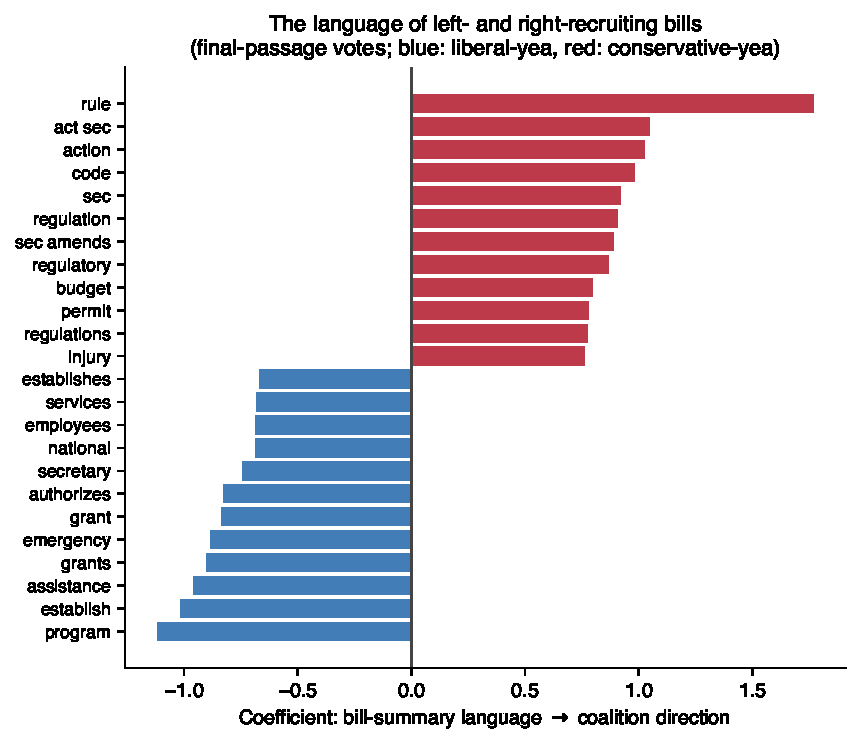
\includegraphics[width=.62\linewidth]{figures/direction_terms.pdf}
\caption{Sparse term-level direction model, final-passage summaries only
(\code{f9}).}
\label{fig:dirterms}
\end{figure}

\subsection{Member-level fit, defection risk, and derived measures}

\textbf{Member fit} (\code{24\_member\_fit.py}): per-member held-out
correct classification and GMP for the 8-D spatial model vs.\
\code{NominateLogit} on identical completion-regime cells, members with
$\ge 100$ held-out votes (Fig.~\ref{fig:membergmp},
Table~\ref{tab:hardcase}). \textbf{Defection scores} (scripts \code{27}
and \code{38}): on majority-yea passage-family rollcalls, each majority
member's predicted defection probability $1 - p_{iv}$; the within-vote
AUC and the member-level risk percentiles of Table~\ref{tab:defectors}
derive from it. \textbf{Embedding diagnostics}
(\code{28\_embedding\_analysis.py}): nearest training-window neighbors
by cosine similarity, restricted to rollcalls preceding the exemplar
(Table~\ref{tab:neighbors}); and the revolt probe, a ridge regression of
majority-defection share on the text embedding alone (holdout
$r = \revoltProbeR$, $n = \revoltProbeN$).

\begin{figure}[tbp]
\centering
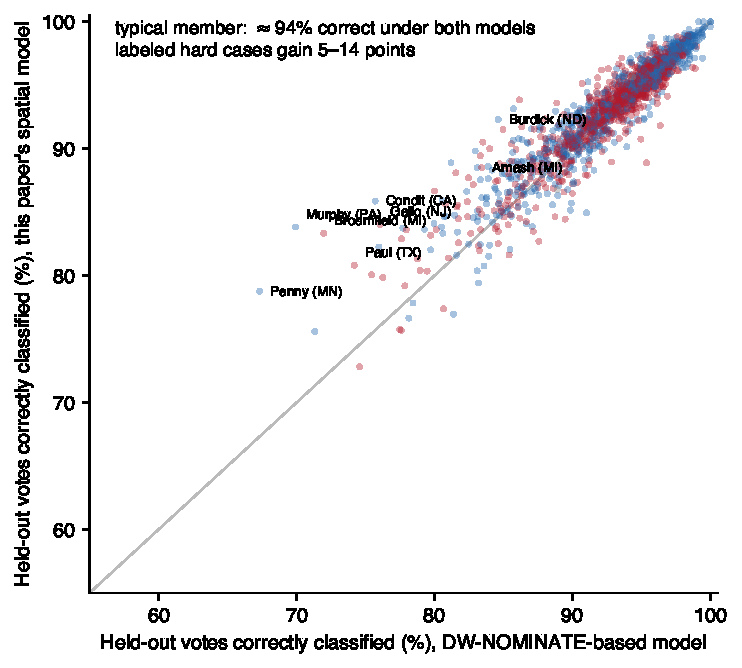
\includegraphics[width=.68\linewidth]{figures/member_cc.pdf}
\caption{Member-level held-out classification, flexible spatial model
vs.\ frozen DW-NOMINATE (\code{24\_member\_fit.py}, \code{f10}).}
\label{fig:membergmp}
\end{figure}

\begin{table}[tbp]
\centering
\caption{Hard-case members, vote by vote (\code{31\_hardcase\_table.py}).}
\label{tab:hardcase}
{\small \begin{tabular}{p{7.2cm}cccc}
\toprule
 & & & \multicolumn{2}{c}{$P(\text{vote cast})$} \\
\cmidrule(lr){4-5}
Held-out vote & Congress & Cast & DW-NOM & This paper \\
\midrule
\multicolumn{5}{l}{\emph{Ron Paul (R-TX)}: 949 held-out votes} \\
\quad National Defense Authorization Act for Fisca\dots & 109 & Nay & 0.00 & 0.99 \\
\quad Intelligence Authorization, FY 1998 & 105 & Nay & 0.00 & 0.99 \\
\quad Electronic Surveillance Modernization Act & 109 & Nay & 0.00 & 0.97 \\
\quad Department of Defense Appropriations Act for\dots & 106 & Nay & 0.02 & 0.99 \\
\quad A concurrent resolution expressing the conce\dots & 108 & Nay & 0.00 & 0.97 \\
\quad Department of Defense Appropriations Act, 20\dots & 109 & Yea & 0.01 & 0.98 \\
\multicolumn{5}{l}{\emph{Justin Amash (MI)}: 579 held-out votes} \\
\quad Providing for consideration of the Senate am\dots & 115 & Nay & 0.01 & 0.94 \\
\quad Reaffirming the United States' commitment to\dots & 112 & Nay & 0.07 & 0.98 \\
\quad To amend the Ronald Reagan Centennial Commis\dots & 112 & Nay & 0.12 & 0.99 \\
\quad Coastal and Great Lakes Communities Enhancem\dots & 116 & Nay & 0.08 & 0.94 \\
\quad John S. McCain National Defense Authorizatio\dots & 115 & Nay & 0.11 & 0.97 \\
\quad Assisting States' Implementation of Plans of\dots & 115 & Nay & 0.11 & 0.96 \\
\bottomrule
\end{tabular}
}
\end{table}

\begin{figure}[tbp]
\centering
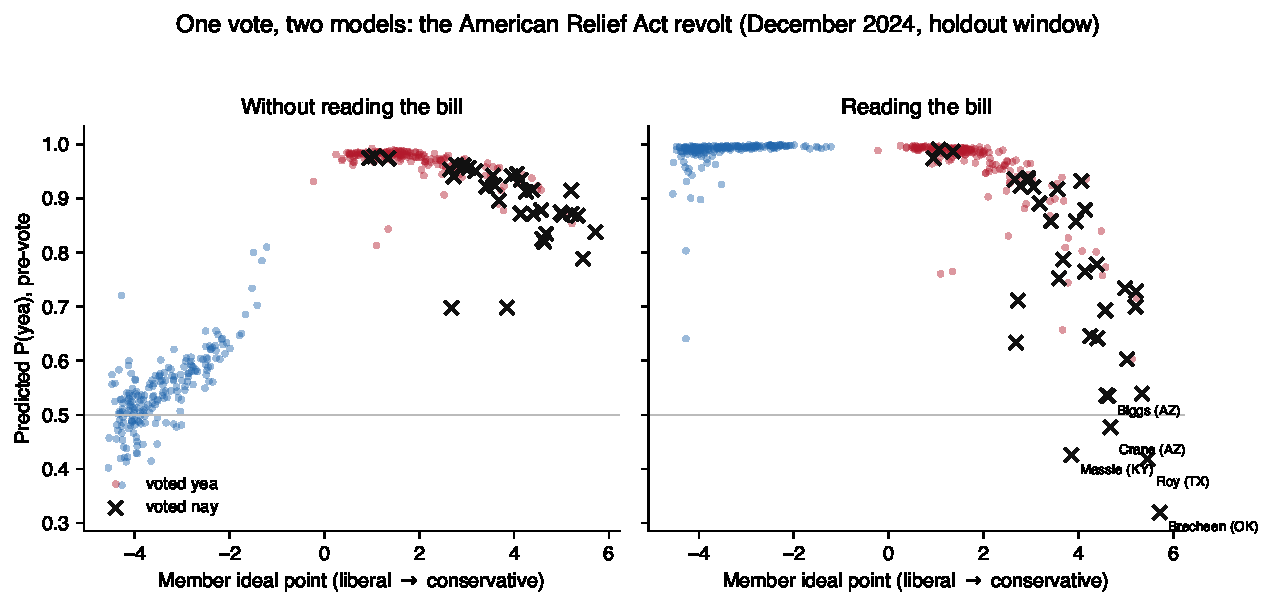
\includegraphics[width=.98\linewidth]{figures/protest_detection.pdf}
\caption{H.R.~10545 predicted by the no-text and text models
(\code{f12}).}
\label{fig:protest}
\end{figure}

\begin{figure}[tbp]
\centering
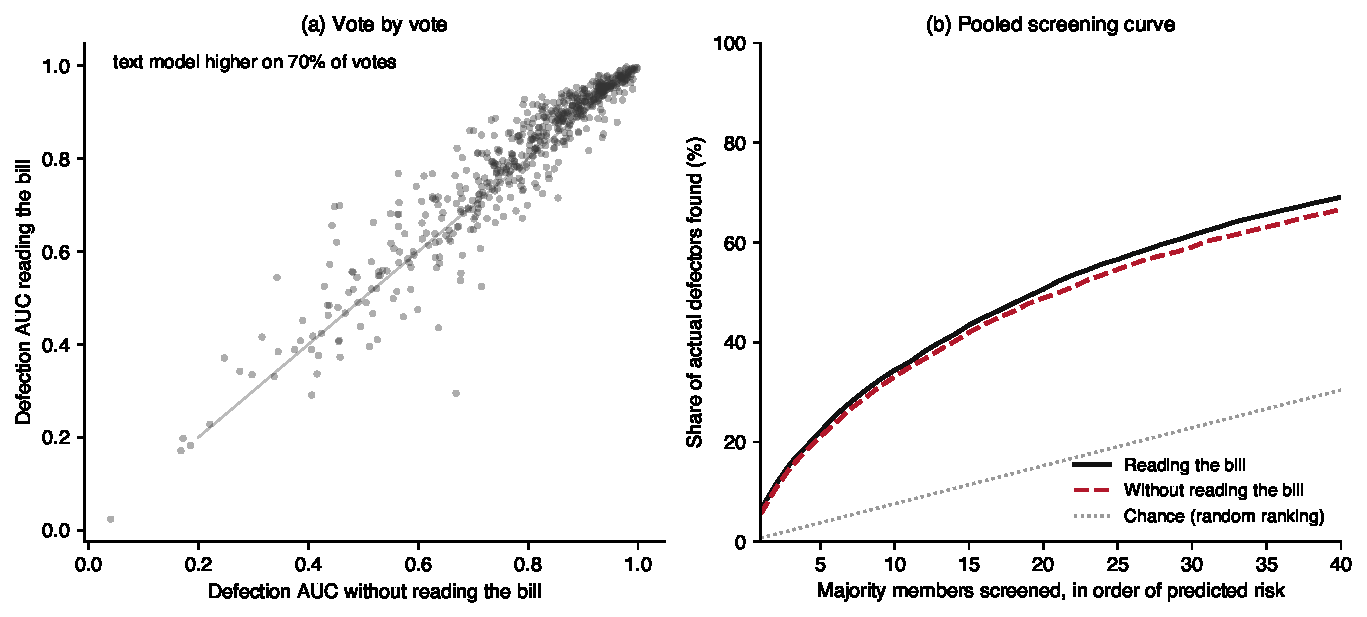
\includegraphics[width=.98\linewidth]{figures/defector_capture.pdf}
\caption{Pooled defection detection (\code{f14}): per-rollcall AUC and
screening curves.}
\label{fig:capture}
\end{figure}

\begin{table}[tbp]
\centering
\caption{Habitual defectors and pre-vote risk percentiles
(\code{38\_defector\_panel.py}).}
\label{tab:defectors}
{\small \begin{tabular}{lcccc}
\toprule
 & & & \multicolumn{2}{c}{Mean pre-vote risk percentile} \\
\cmidrule(lr){4-5}
Member & Defections & Rate & Text model & No-text \\
\midrule
\multicolumn{5}{l}{\emph{Republican majorities (top 8 by defection rate)}} \\
\quad Rosendale (R-MT) & 71 & 56\% & 97 & 96 \\
\quad Roy (R-TX) & 87 & 52\% & 99 & 97 \\
\quad Good (R-VA) & 63 & 48\% & 93 & 92 \\
\quad Paul (R-TX) & 103 & 48\% & 99 & 99 \\
\quad Biggs (R-AZ) & 120 & 46\% & 98 & 97 \\
\quad Greene (R-GA) & 51 & 45\% & 97 & 95 \\
\quad Massie (R-KY) & 177 & 42\% & 99 & 98 \\
\quad Amash (R-MI) & 122 & 41\% & 98 & 98 \\
\multicolumn{5}{l}{\emph{Democratic majorities (top 8 by defection rate)}} \\
\quad Bright (D-AL) & 22 & 35\% & 99 & 98 \\
\quad Feingold (D-WI) & 19 & 26\% & 89 & 92 \\
\quad Adler (D-NJ) & 17 & 24\% & 91 & 95 \\
\quad Minnick (D-ID) & 16 & 23\% & 99 & 99 \\
\quad Shuler (D-NC) & 38 & 22\% & 94 & 94 \\
\quad Nye (D-VA) & 15 & 19\% & 96 & 93 \\
\quad Byrd (D-WV) & 9 & 19\% & 81 & 82 \\
\quad Kratovil (D-MD) & 14 & 18\% & 97 & 99 \\
\multicolumn{5}{l}{\emph{The modern left flank (named cases; 116th--117th windows)}} \\
\quad Tlaib (D-MI) & 17 & 9\% & 96 & 95 \\
\quad Ocasio-Cortez (D-NY) & 15 & 8\% & 93 & 94 \\
\quad Bush (D-MO) & 9 & 8\% & 99 & 92 \\
\quad Omar (D-MN) & 12 & 6\% & 92 & 93 \\
\quad Pressley (D-MA) & 11 & 6\% & 93 & 93 \\
\bottomrule
\end{tabular}
}
\end{table}

\begin{table}[tbp]
\centering
\caption{Embedding-space nearest neighbors
(\code{28\_embedding\_analysis.py}).}
\label{tab:neighbors}
{\small \begin{tabular}{p{7.8cm}ccc}
\toprule
Nearest earlier bills in the encoder's text space & Congress & \shortstack{Text\\similarity} & \shortstack{Its majority\\defection} \\
\midrule
\multicolumn{4}{l}{\emph{American Relief Act (CR), Dec.\ 2024}: realized majority defection 17\%} \\
\quad Tax Relief for American Families and Workers & 118 & 0.81 & 22\% \\
\quad Federal Disaster Tax Relief Act & 118 & 0.81 & 4\% \\
\quad Further Continuing Appropriations and Other  & 118 & 0.74 & 42\% \\
\multicolumn{4}{l}{\emph{Social Security Fairness Act, Nov.\ 2024}: realized majority defection 34\%} \\
\quad Securing a Strong Retirement Act of 2022 & 117 & 0.69 & 0\% \\
\quad NDO Fairness Act & 118 & 0.68 & 0\% \\
\quad Tax Relief for American Families and Workers & 118 & 0.68 & 22\% \\
\multicolumn{4}{l}{\emph{BIOSECURE Act, Sept.\ 2024}: realized majority defection 1\%} \\
\quad Preventing the Financing of Illegal Syntheti & 118 & 0.70 & 1\% \\
\quad Pro Codes Act & 118 & 0.70 & 26\% \\
\quad Food and Drug Administration Amendments Act  & 110 & 0.69 & 1\% \\
\bottomrule
\end{tabular}
}
\end{table}

\begin{figure}[tbp]
\centering
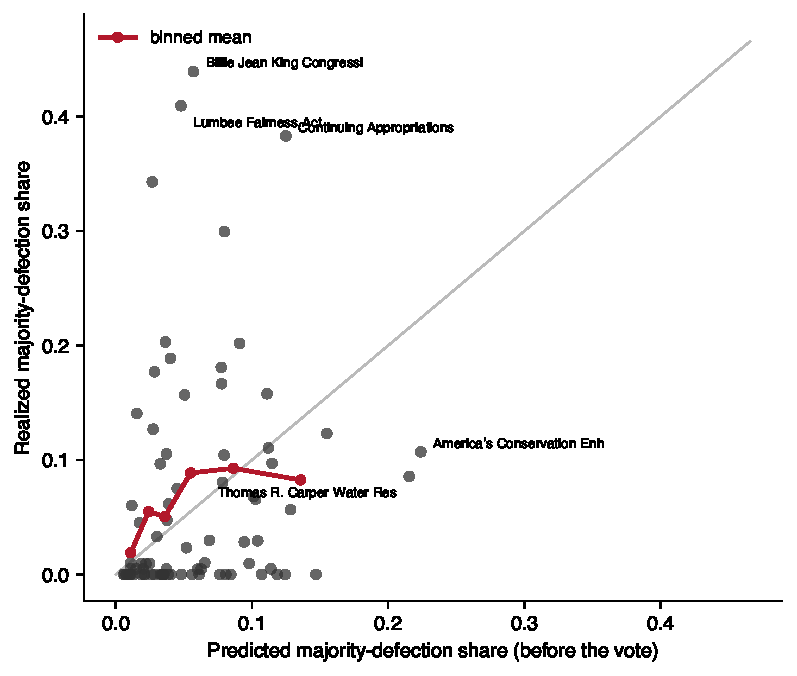
\includegraphics[width=.62\linewidth]{figures/revolt_risk.pdf}
\caption{Pre-vote revolt-risk index vs.\ realized defection, 118th House
holdout (\code{f13}).}
\label{fig:revoltrisk}
\end{figure}

%=====================================================================
\section{Validation and robustness}
\label{sec:validation}

\subsection{Feature-timing audit and the leakage-clean specification}
\label{sec:leakage}

Per-field timing rules: vote question and description, fixed at the vote
(no earlier timestamp exists); bill title and sponsor, fixed at
introduction; bill summaries, only versions with CRS action dates
strictly before the vote date; amendment purpose and amender party,
filed at submission, joined with session-offset verification;
member-by-question rates, training window only; early stopping and
calibration, the final 5\% of training rollcalls, strictly inside train.
CRS legislative-subject terms are revisable without version history; the
TF--IDF ensemble component uses them, so the fully conservative headline
is the single MiniLM tower (\incForecastLL{} log loss) beside the
ensemble (\champForecastLL); the protest comparison is likewise reported
leakage-clean (within-vote AUC \protAUCclean{} vs.\ \protAUCnotext{}
no-text), and the cutpoint headline feature set contains no revisable
fields.

\subsection{The prospective protocol}
\label{sec:prospective}

\code{13\_freeze\_model.py}/\code{20\_freeze\_model\_v2.py} pickle the
fitted artifact and record its SHA-256, training-data snapshot date, and
registry configuration in a metadata JSON. The scoring scripts
(\code{14\_score\_prospective.py} and its v2 counterpart,
\code{21\_score\_prospective\_v2.py}) verify the hash before every use
and score only member-votes cast after the snapshot. The pickle is never
modified (backward-compatible attribute defaults are class-level, so old
artifacts deserialize unchanged). v1 (June 12, 2026 freeze):
\prospectiveVoneLL{} log loss on \prospectiveN{} post-snapshot decisions
across \prospectiveRC{} rollcalls, \postFreezeLL{} on the strictly
post-freeze subset; v2 (July 3): accumulating. The audit is small by
construction and labeled preliminary; it exists because temporal
holdouts are reusable and iteration can overfit them
\citep{dwork2015holdout}.

\begin{table}[tbp]
\centering
\caption{Frozen-artifact scoring.}
\label{tab:prospective}
\begin{tabular}{llrrccc}
\toprule
Artifact & Snapshot & Rollcalls & Votes & Log loss & Acc.\ (\%) & AUC \\
\midrule
v1 (emb2-MLP tower) & 2026-06-09 & 43 & 9,451 & 0.331 & 85.7 & 0.924 \\
v2 (three-tower blend) & 2026-06-09 & 43 & 9,451 & 0.332 & 86.8 & 0.921 \\
\bottomrule
\end{tabular}

\end{table}

\subsection{Stratified evaluations (\code{29\_stratified\_eval.py})}

Seen-bill vs.\ fresh-bill: a held-out rollcall is ``seen'' if its bill
had any rollcall in the training partition; the text gain is larger on
fresh bills (\freshLLchamp{} vs.\ \freshLLnotext{} no-text, over
\freshRC{} rollcalls) than seen ones (\seenLLchamp{} vs.\ \seenLLnotext,
\seenRC), refuting bill-family recall as the mechanism. Chamber: House
\houseLLchamp{} vs.\ \houseLLnotext; Senate \senateLLchamp{} vs.\
\senateLLnotext. Policy-area text gains (Table~\ref{tab:policygain}) use
CRS policy area as an evaluation stratifier only.

\begin{table}[tbp]
\centering
\caption{Text gain by policy area (no-text minus model log loss).}
\label{tab:policygain}
{\small \begin{tabular}{lccc}
\toprule
Policy area & Held-out rollcalls & \multicolumn{2}{c}{Text gain in log loss} \\
 & & Ensemble & Clean tower \\
\midrule
Government Operations and Politics & 64 & +0.103 & +0.094 \\
International Affairs & 40 & +0.090 & +0.075 \\
Public Lands and Natural Resources & 46 & +0.075 & +0.062 \\
Armed Forces and National Security & 90 & +0.051 & +0.059 \\
Transportation and Public Works & 26 & +0.044 & +0.035 \\
Economics and Public Finance & 51 & +0.012 & +0.017 \\
Crime and Law Enforcement & 58 & +0.058 & +0.011 \\
Energy & 28 & +0.044 & +0.005 \\
Health & 50 & +0.052 & -0.006 \\
Taxation & 43 & +0.042 & -0.021 \\
Congress & 165 & -0.006 & -0.028 \\
Finance and Financial Sector & 43 & +0.022 & -0.070 \\
\bottomrule
\end{tabular}
}
\end{table}

\subsection{Redaction ablations and counterfactual edits}
\label{sec:ablation}

\code{30\_text\_ablation.py} rebuilds every legislation-linked holdout
rollcall's exact text template, applies a redaction, re-embeds with the
identical encoder, swaps the embedding into the frozen champion's MiniLM
tower \emph{in memory} (the artifact on disk is untouched and
hash-verified), and re-scores the identical member-vote cells---so all
non-text inputs are held fixed and differences isolate the text
component. Variants: summary removed; question removed; titles replaced
by generic language; proper nouns masked (capitalized sequences and
acronyms); digits removed; and the placebo, description + bill text
replaced by a random different holdout bill's from the same policy area
and question bucket (seeded RNG). \code{34\_counterfactual\_edits.py}
applies targeted edits to exemplars through the same machinery
(Table~\ref{tab:counterfactual}); exemplar selection rules (title-only
CR; highest-predicted-defection summary-rich vote) are stated in the
script header.

\begin{table}[tbp]
\centering
\caption{Redaction ablations through the frozen tower
(\code{30\_text\_ablation.py}).}
\label{tab:ablation}
{\small \begin{tabular}{lccc}
\toprule
Text given to the frozen model & Log loss & $\Delta$ & Defection AUC \\
\midrule
Original text & 0.328 &  & 0.784 \\
Bill summary removed & 0.351 & +0.023 & 0.811 \\
Vote question removed & 0.383 & +0.055 & 0.766 \\
Titles replaced by generic language & 0.340 & +0.012 & 0.768 \\
Proper nouns masked & 0.339 & +0.011 & 0.779 \\
Digits removed & 0.328 & +0.000 & 0.787 \\
Text from another bill, same policy area & 0.392 & +0.064 & 0.777 \\
\bottomrule
\end{tabular}
}
\end{table}

\begin{table}[tbp]
\centering
\caption{Counterfactual text edits (\code{34\_counterfactual\_edits.py}).}
\label{tab:counterfactual}
{\small \begin{tabular}{p{7.6cm}ccc}
\toprule
Text supplied to the frozen model & \shortstack{Predicted\\defection share} & \shortstack{Implied\\defectors} & \shortstack{Top-5 picks\\who defected} \\
\midrule
\multicolumn{4}{l}{\emph{American Relief Act CR, Dec.\ 2024 (pre-vote text is title-only)}} \\
\multicolumn{4}{l}{\quad\emph{realized outcome: 34 of 204 majority members defected (17\%)}} \\
\quad Original (title + suspension question) & 6.5\% & 13 & 5/5 \\
\quad Title replaced by generic language & 2.7\% & 6 & 5/5 \\
\quad Question changed to On Passage & 13.5\% & 28 & 5/5 \\
\quad BIOSECURE Act title substituted & 8.4\% & 17 & 5/5 \\
\multicolumn{4}{l}{\emph{Appalachian Regional Development Act Amendments, 2006 (full pre-vote summary)}} \\
\multicolumn{4}{l}{\quad\emph{realized outcome: 55 of 223 majority members defected (25\%)}} \\
\quad Original (title + summary) & 14.5\% & 32 & 5/5 \\
\quad Spending-program sentences removed & 14.7\% & 33 & 5/5 \\
\quad Generic title, summary kept & 12.6\% & 28 & 4/5 \\
\quad Same-area bill's summary substituted & 7.3\% & 16 & 4/5 \\
\bottomrule
\end{tabular}
}
\end{table}

\subsection{Calibration}

Reliability curves, Brier scores, and 15-bin ECE for ensemble
(\brierChamp/\eceChamp), clean tower (\brierClean/\eceClean), and
no-text (\brierNotext/\eceNotext); rollcall-level defection-share
calibration by decile (predicted--realized correlation \defShareRChamp{}
vs.\ \defShareRNotext).

\begin{figure}[tbp]
\centering
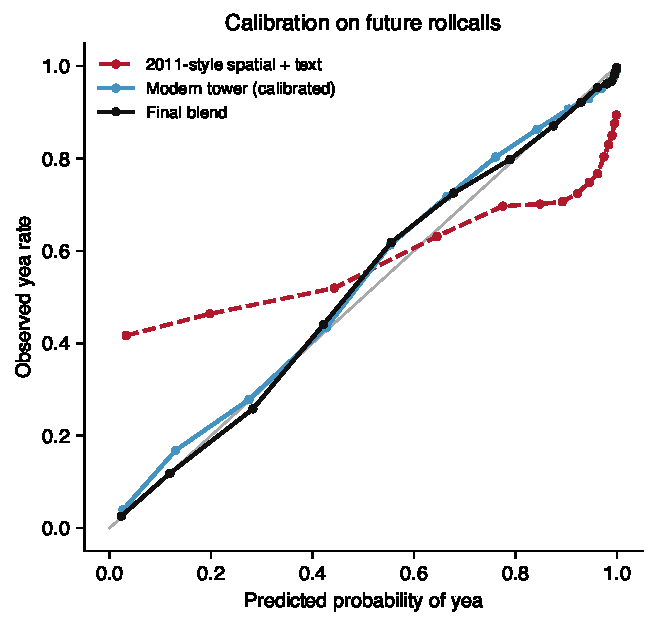
\includegraphics[width=.95\linewidth]{figures/calibration.pdf}
\caption{Member-vote reliability and defection-share calibration
(\code{32\_calibration\_metrics.py}, \code{f6}).}
\label{fig:calibration}
\end{figure}

\subsection{Majority transitions and amendment experiments}

\code{25\_transitions.py}: for every adjacent House congress pair, train
through the earlier congress, score the later; flips vs.\ placebo
(no-flip) transitions, overall and by vote type. Procedural transfer
degrades at every flip and no placebo (\flipProcLL{} vs.\ \placeboProcLL{}
mean log loss; event-level points in Fig.~\ref{fig:transitions});
final-passage transfer is flip-invariant (\flipPassLL{} vs.\
\placeboPassLL). Amendment-text experiments (ledger E5a--c): three
feature variants plus a placebo in which the amendment-text file is
rebuilt with permuted assignments---the pre-registered falsification
test that the join itself, not the language, carries any effect; text
variants score \eFiveA/\eFiveB/\eFiveC{} against control \champValCtrl{}
and placebo \eFivePlacebo{} on validation, so purpose text is excluded
from all registered models while the amender's \emph{party} enters the
cutpoint metadata.

\begin{figure}[tbp]
\centering
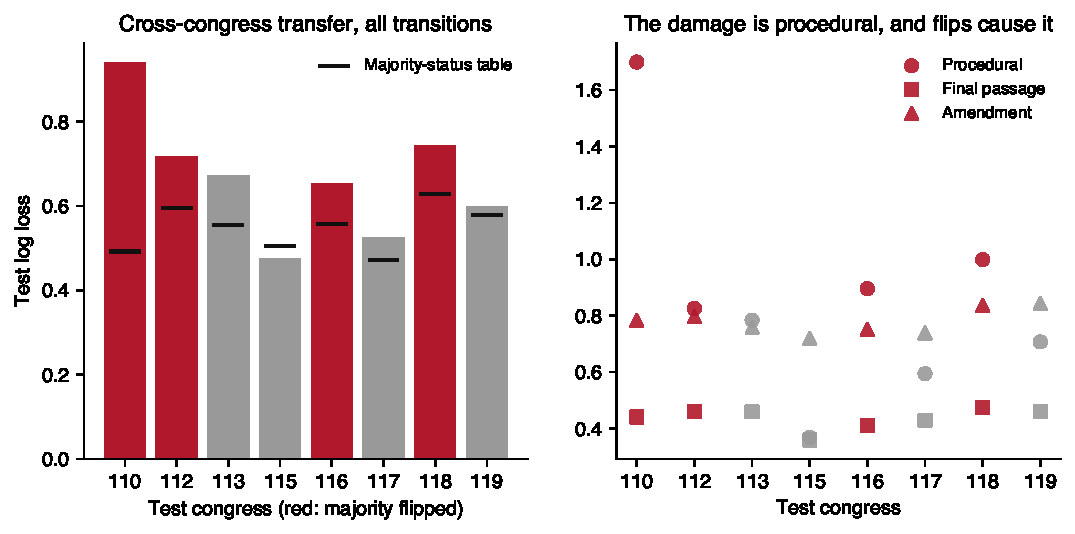
\includegraphics[width=.95\linewidth]{figures/transitions.pdf}
\caption{Cross-congress transfer at every House transition
(\code{25\_transitions.py}, \code{f11}).}
\label{fig:transitions}
\end{figure}

\subsection{Member-level cross-checks}

\code{33\_member\_overlap.py}: Spearman rank correlation between member
scaling gains (completion regime) and member defection-pricing gains
(forecast regime) is $\rho = \overlapRho$ over \overlapN{}
members---the two improvements are related at the level of the
phenomenon, not member by member; this check corrected an earlier
overclaim in draft text. Convergent validity: first-dimension positions
vs.\ DW-NOMINATE $r=.98$; vs.\ Nokken--Poole per congress
$r = \npRmin$--$\npRmax$.

\subsection{The experiment ledger}

\begin{table}[tbp]
\centering
\caption{Ledger audit trail (full record with timestamps in
\code{Notes/experiment\_ledger.md}).}
\label{tab:ledger}
{\small
\begin{tabular}{llll}
\toprule
ID & Hypothesis & Falsification test & Outcome \\
\midrule
M-A & bigger encoder helps long bills & long-bill val loss falls & negative \\
E1 & within-bill context helps & beats shuffled-bill placebo & negative \\
E1b & stacked context corrector & permuted-bill weights $\to 0$ & null \\
E2 & recency-weighted rates help & $\tau\to\infty$ recovers flat & negative \\
E3 & per-bucket calibration helps & val loss below global cal. & negative \\
E4/E4b & tower blends help & dev-weight collapse if redundant & positive \\
E4b(r) & dev-slice params inherit regime & interleaved val degrades & confirmed \\
E5a--c & amendment text helps & beats placebo file rebuild & negative \\
S5 & blend beats champion & one-shot test LL below champion & positive \\
\bottomrule
\end{tabular}}
\end{table}

Negative results with diagnosed mechanisms, in addition to the table:
encoder scale (a $16\times$ text budget does not help and hurts long
bills); within-bill context features (shortcut learning starves the
backbone; the E1b stacked corrector was cleanly null); recency weighting
of member rates; per-bucket calibration; and the GBSpatial memory
incident (a $(n,1)\times(n)$ broadcast in scikit-learn ridge prediction
at $k=1$ produced an $(n,n)$ allocation---fixed with shape asserts and a
production-configuration test, and recorded as a process lesson).

%=====================================================================
\section{Code map}
\label{sec:code}

\begin{center}
{\footnotesize
\begin{tabular}{lp{8.6cm}}
\toprule
Script & Function \\
\midrule
\code{00--01} & download Voteview; build the vote panel \\
\code{02, 06, 12, 17} & construct the four split families (hash/temporal) \\
\code{04, 05, 07, 16, 18} & BILLSTATUS fetch/parse; bill, cosponsor,
amendment joins \\
\code{08, 19} & rollcall text templates and sentence embeddings (v2/v3) \\
\code{03, 09--11} & positions, member signals, issue positions/probes \\
\code{13--14, 20--21} & freeze and score prospective artifacts (v1, v2) \\
\code{22--24} & measures: cutpoints, cutpoint prediction, member fit \\
\code{25--28} & transitions, worked example, protest detection,
embeddings \\
\code{29--35, 37--38} & review-driven diagnostics: stratified evaluation,
redaction ablations, hard cases, calibration, overlap, counterfactual
edits, cutpoint strata, benchmark card, defector panel \\
\code{models\_*.py} & model classes and registries \\
\code{harness.py}, \code{run\_benchmark.py} & metrics, label stripping,
leaderboard \\
\code{make\_tables.py}, \code{make\_figures.py} & every exhibit and
macro in both documents \\
\code{dashboard\_app.py} & interactive forecaster (single-tower
approximation) \\
\bottomrule
\end{tabular}}
\end{center}

Reproducibility invariants: all statistics enter the documents as
generated macros or \code{\textbackslash input} tables
(\code{make\_tables.py} fails loudly on placeholder cells); split files
and frozen artifacts are content-hashed; conversation-level session logs
and the experiment ledger are part of the repository. The headline table
reproduces in under two GPU-hours on a laptop-class accelerator; the
benchmark runs one model per process (\S\ref{sec:regimes}).

\bibliographystyle{apsr}
\bibliography{references}

\end{document}
